\section{Trénování hlubokého modelu variačního autoenkodéru}
Trénovací fáze modelu variačního autoenkodéru spočívá v minimalizaci ztrátové funkce dle \autoref{sec:vae_model_loss_function}.
Účelem této ztrátové funkce je současná minimalizace chyby rekonstrukce a regularizace naučené pravděpodobnostní distribuce latentních proměnných za účelem přiblížení k apriorní distribuci vstupních dat.
Pro umožnění zpětné propagace byla představena reparametrizační vrstva modelu variačního autoenkodéru, která činí vzorkovací proces diferenciovatelným.

Trénovací proces sestaveného modelu lze zahájit následovně\footnote{Optimizer Adam slouží pro stochastickou gradientní optimalizaci dle \autoref{sec:stochastic_gradient_optimization_method}.}:
\lstinputlisting[language=Python, caption=Zahájení testovací fáze modelu variačního autoenkodéru pro úlohu generativního modelování obrazových dat MNIST.]{code_snippets/vae_train.py}

Vstupem pro trénování modelu jsou trénovací data MNIST (\lstinline{x_train}). Způsob jejich načtení a předzpracování je dostupný v \autoref{app:vae_model_source_code}.

\newpage
\subsection{Konvergence ztrátové funkce}
Počet epoch trénovací fáze modelu byl empiricky stanoven na 200. \autoref{app:latent_space_development} prezentuje formulaci latentního prostoru modelu variačního autoenkodéru s různým počtem epoch.
\begin{figure}[H]
    \centering
    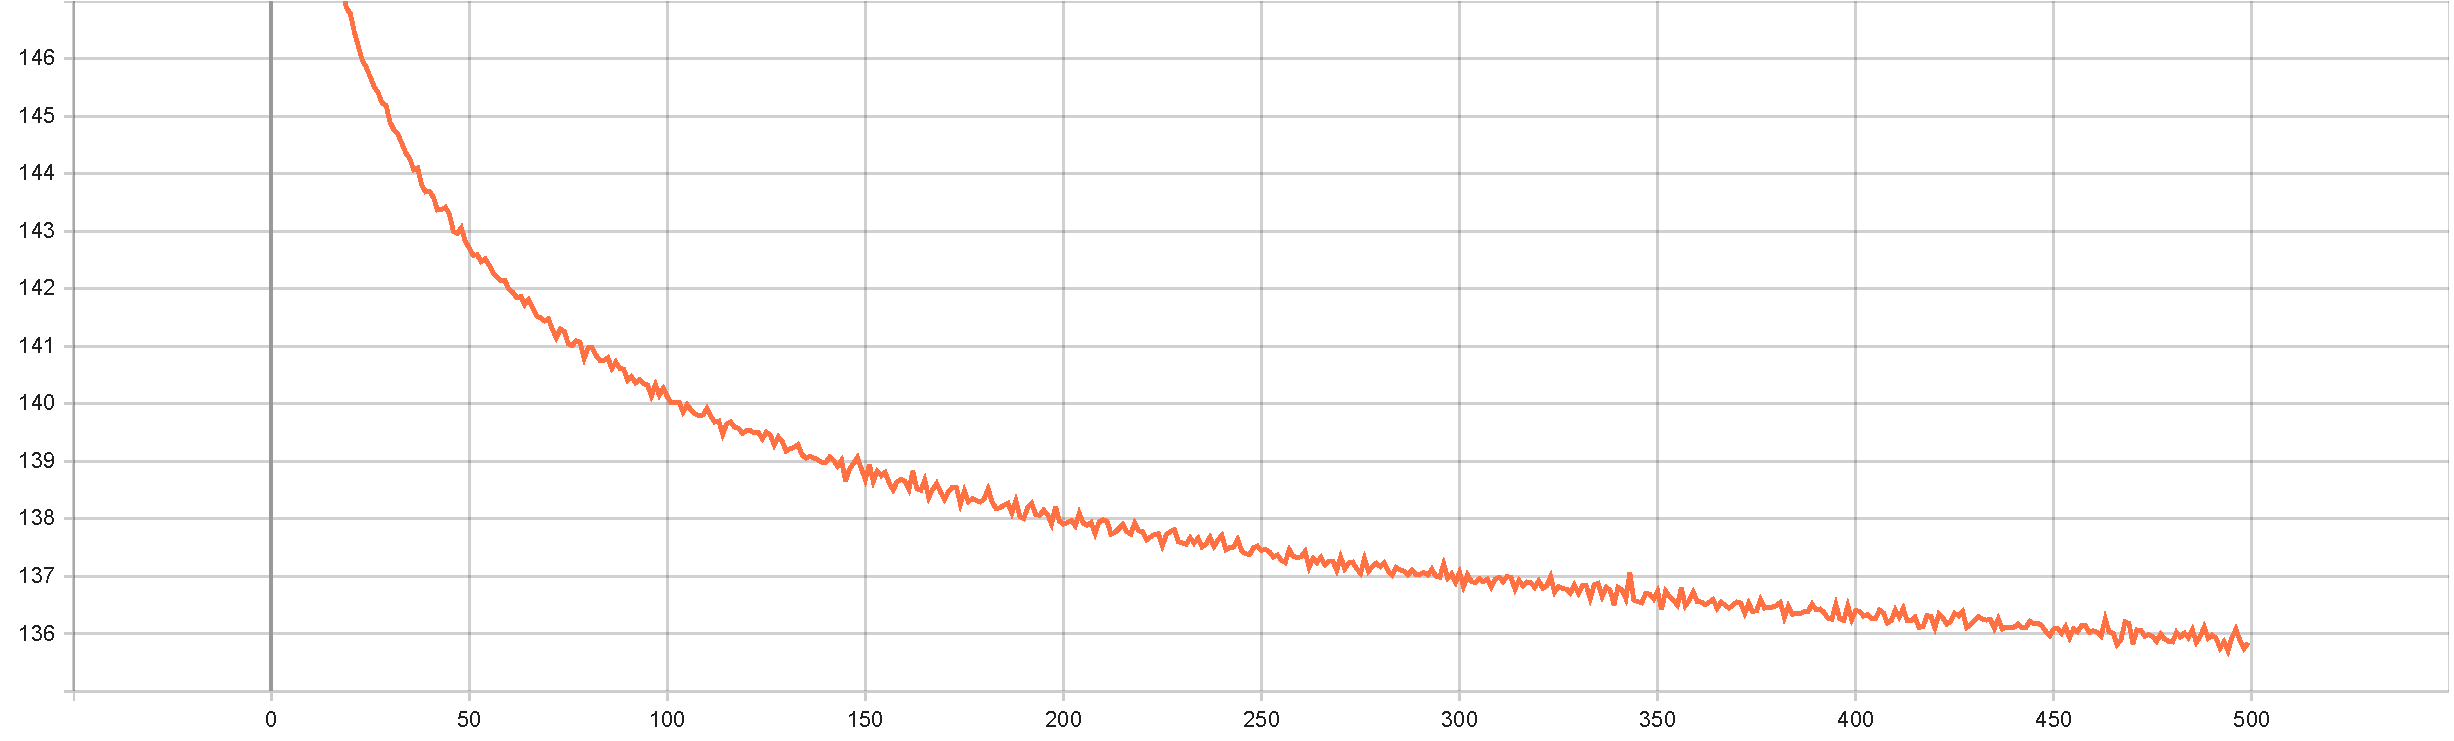
\includegraphics[width=0.97\textwidth]{figures/vae_model_total_loss_500_epochs.pdf}
    \caption{Ztrátová funkce po 500 epochách konverguje k hodnotě $\sim 135.8$. Osa x značí počet epoch. Osa y značí hodnotu ztrátové funkce.}
\end{figure}

\begin{figure}[H]
    \centering
    \subfloat[\centering KL divergence po 500 epochách konverguje k hodnotě $\sim 3.8$.]{{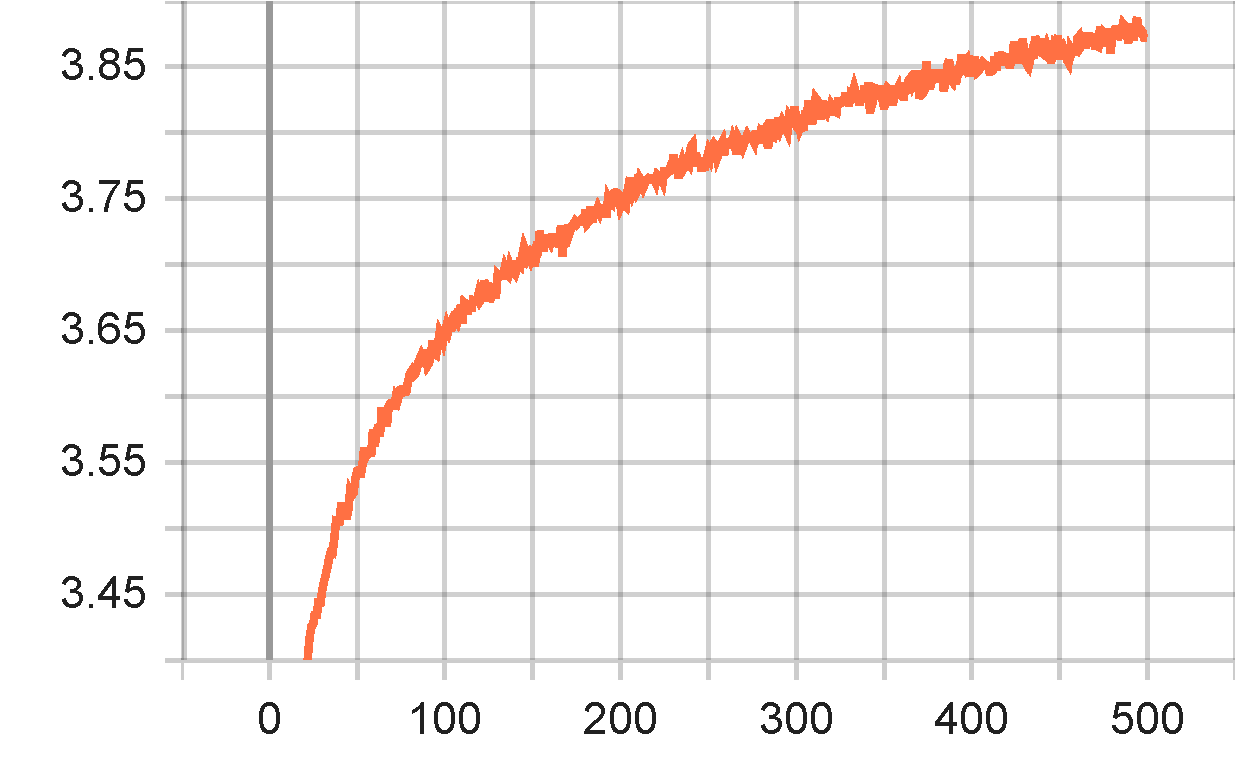
\includegraphics[width=0.45\textwidth]{figures/vae_model_kl_loss_500_epochs.pdf} }}
    \qquad
    \subfloat[\centering Chyba rekonstrukce po 500 epochách konverguje k hodnotě $\sim 132$.]{{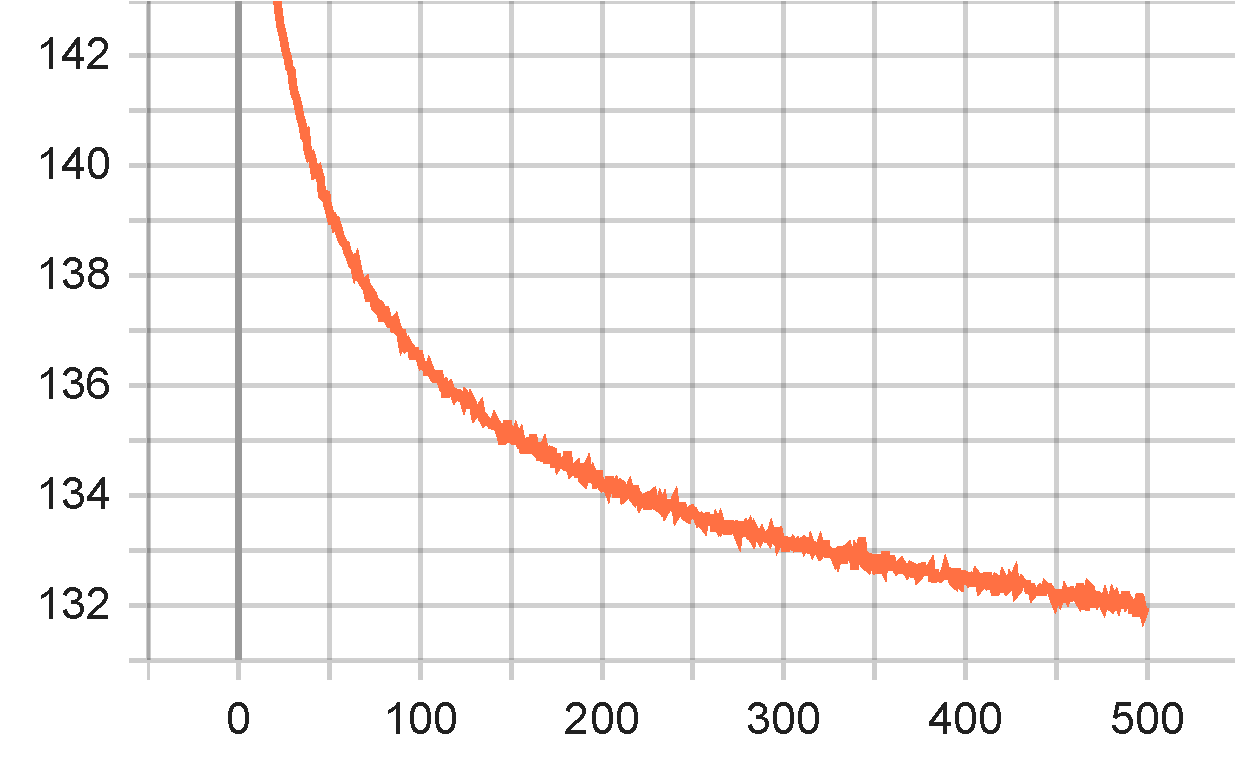
\includegraphics[width=0.45\textwidth]{figures/vae_model_reconstruction_loss_500_epochs.pdf} }}
    \caption{Hodnoty dílčích prvků ztrátové funkce modelu variačního autoenkodéru po 500 epochách. Osa x značí počet epoch. Osa y značí hodnotu dílčího prvku ztrátové funkce.}
    \label{fig:example}
\end{figure}

Počet epoch byl na základě doménové znalosti (tedy předem známý počet tříd a sémantické vztahy mezi nimi) a postupného formování latentního prostoru, jak zachycuje \autoref{fig:forming_latent_space} stanoven na \textbf{500}.
Při vizualizaci latentního prostoru modelu, jehož trénovací fáze obsahovalo 500 epoch lze pozorovat emergenci struktury v latentní prostoru, která koresponduje se skutečným významem trénovacích dat (číslice 0-9, 10 skupin) a trénovací fáze tak v tomto bodě byla ukončena.

\subsection{Možné zlepšení trénovací strategie variačního autoenkodéru}
Variační autoenkodér při trénování balancuje dva prvky ztrátové funkce (viz \autoref{eq:vae_elbo}) – chybu rekonstrukce a KL divergenci.
Usměrnění těchto dvou prvku lze dosáhnout zahrnutím hyperparametru $\beta$ do trénovací fáze modelu. 
Tento hypermarametr má skalární hodnota a slouží k násobení KL divergence prvku ztrátové funkce, tedy přiděluje KL divergenci váhu.

Je-li $\beta = 1$, pak variační autoenkodér optimalizuje efekt chyby rekonstrukce i KL divergence rovnocenně.   
Je-li $\beta < 1$, dává variační autoenkodér větší důraz na minimalizaci chyby rekonstrukce.
Je-li $\beta > 1$, dává variační autoenkodér naopak větší důraz na regularizační efekt KL divergence.

V této ilustrační implementaci generativního modelu MNIST pro jednoduchost \textbf{hyperparemetr $\beta$ nebyl součástí trénovacího procesu}.
Jeho začlenění by však vedlo k ještě lépe struktorovanému latentnímu prostoru naučeného modelu, než prezentuje \autoref{fig:forming_latent_space}.

U složitějších modelů variačního autoenkodéru nalézá uplatnění $\beta$ hyperparametru úspěch.
Výzkumníci \textcite{Tomczak2017} dokonce přichází se strategií postupného žíhání hodnoty $\beta$.
Začínají s hodnotou $\beta = 0.1$ a postupně ji zvyšují.
To v důsledku umožní modelu se v úvodní fázi trénování zaměřit na minimalizaci chyby rekonstrukce.
V pozdější fázi trénovacího procesu je naopak postupně upřednostňován regularizační efekt KL divergence, což ve finále vede k přesnějšímu zachycení struktury dat a zamezuje přeučení.

